\section{Experiments}
\seclabel{experiments}

\TODO{All experiments here are preliminary. Add new results from more objects, especially non-symmetric ones.} \\
\TODO{Include experiments on sensitivity to uncertainty.} \\
\TODO{Images of selected grasps.} \\

We evaluated the convergence rate of Algorithm~\ref{alg:full} for varying sizes of prior data used from Dex-Net and examined the sensitivity of the convergence rate to the kernel bandwidths, number of nearest neighbors, and uncertainty.
We created three nested training sets of 100, 1000, and 10000 objects by uniformly sampling objects from Dex-Net.
From the remaining objects we created a set of 20 validation objects for selecting algorithm hyperparameters and a set of 30 objects for test data.
We used isotropic covariance with object and gripper translation variance $\sigma_{t} = 0.005$, object and gripper rotation variance $\sigma_{r} = 0.1$, and friction variance $\sigma_{\gamma} = 0.1$.
The bandwidths of our similarity kernel were set to scaling transformations $C = \sigma I$ where $\sigma \in \bR$ for the grasp parameter and global object feature maps, and a gaussian mask $C_d$ centered on the gradient heightmaps with height $w_d \in \bR$ and variance $\sigma_d \in \bR$.
The bandwidths were selected by maximizing convergence rate on the validation set using a grid search over hyperparameters.

To handle the scale of the experiments, we developed a Cloud-based software library on top of Google Cloud Platform.
We used Google Compute Engine to distribute trials of MAB algorithms across objects and Google Cloud Storage (GCS) to store Dex-Net.
Our experimental scripts launched up to 1500 GCE single core instances at one time for hyperparameter tuning and convergence analysis, reducing the runtime of our experiments by a factor of nearly $1500\times$.

\subsection{Rate of Convergence}
\TODO{Replace with final versions. The current results are preliminary}

~\figref{local-mab} shows the normalized $P_F$ (the ratio of the $P_F$ for the sampled grasp to the highest $P_F$ in the candidate grasp set) versus iteration averaged over 20 trials for a cereal box and flower pot.
The plot compares Algorithm~\ref{alg:full} with no prior data to uncorrelated Thompson sampling and uniform allocation, two methods used by Laskey et al.~\cite{laskey2015bandits}.
We see that the CCBP model outperforms the uncorrelated model by approximately 10$\times$ for the cereal box but has comparable performance to Thompson sampling on the flower pot.
Iniitial reuslts suggest that performance on the flower pot is poorer because few grasps are similar according to our feature representation.

%Preliminary experiments suggest that using CCBPs with prior data from DexNet reduces the number of samples for MAB algorithms to converge to a grasp with high probablity of force closure $P_F$ under uncertainty in object pose, gripper pose, and friction coefficient.

\begin{figure}[t!]
\centering
	\begin{subfigure}[b]{0.5\textwidth}
        \centering
        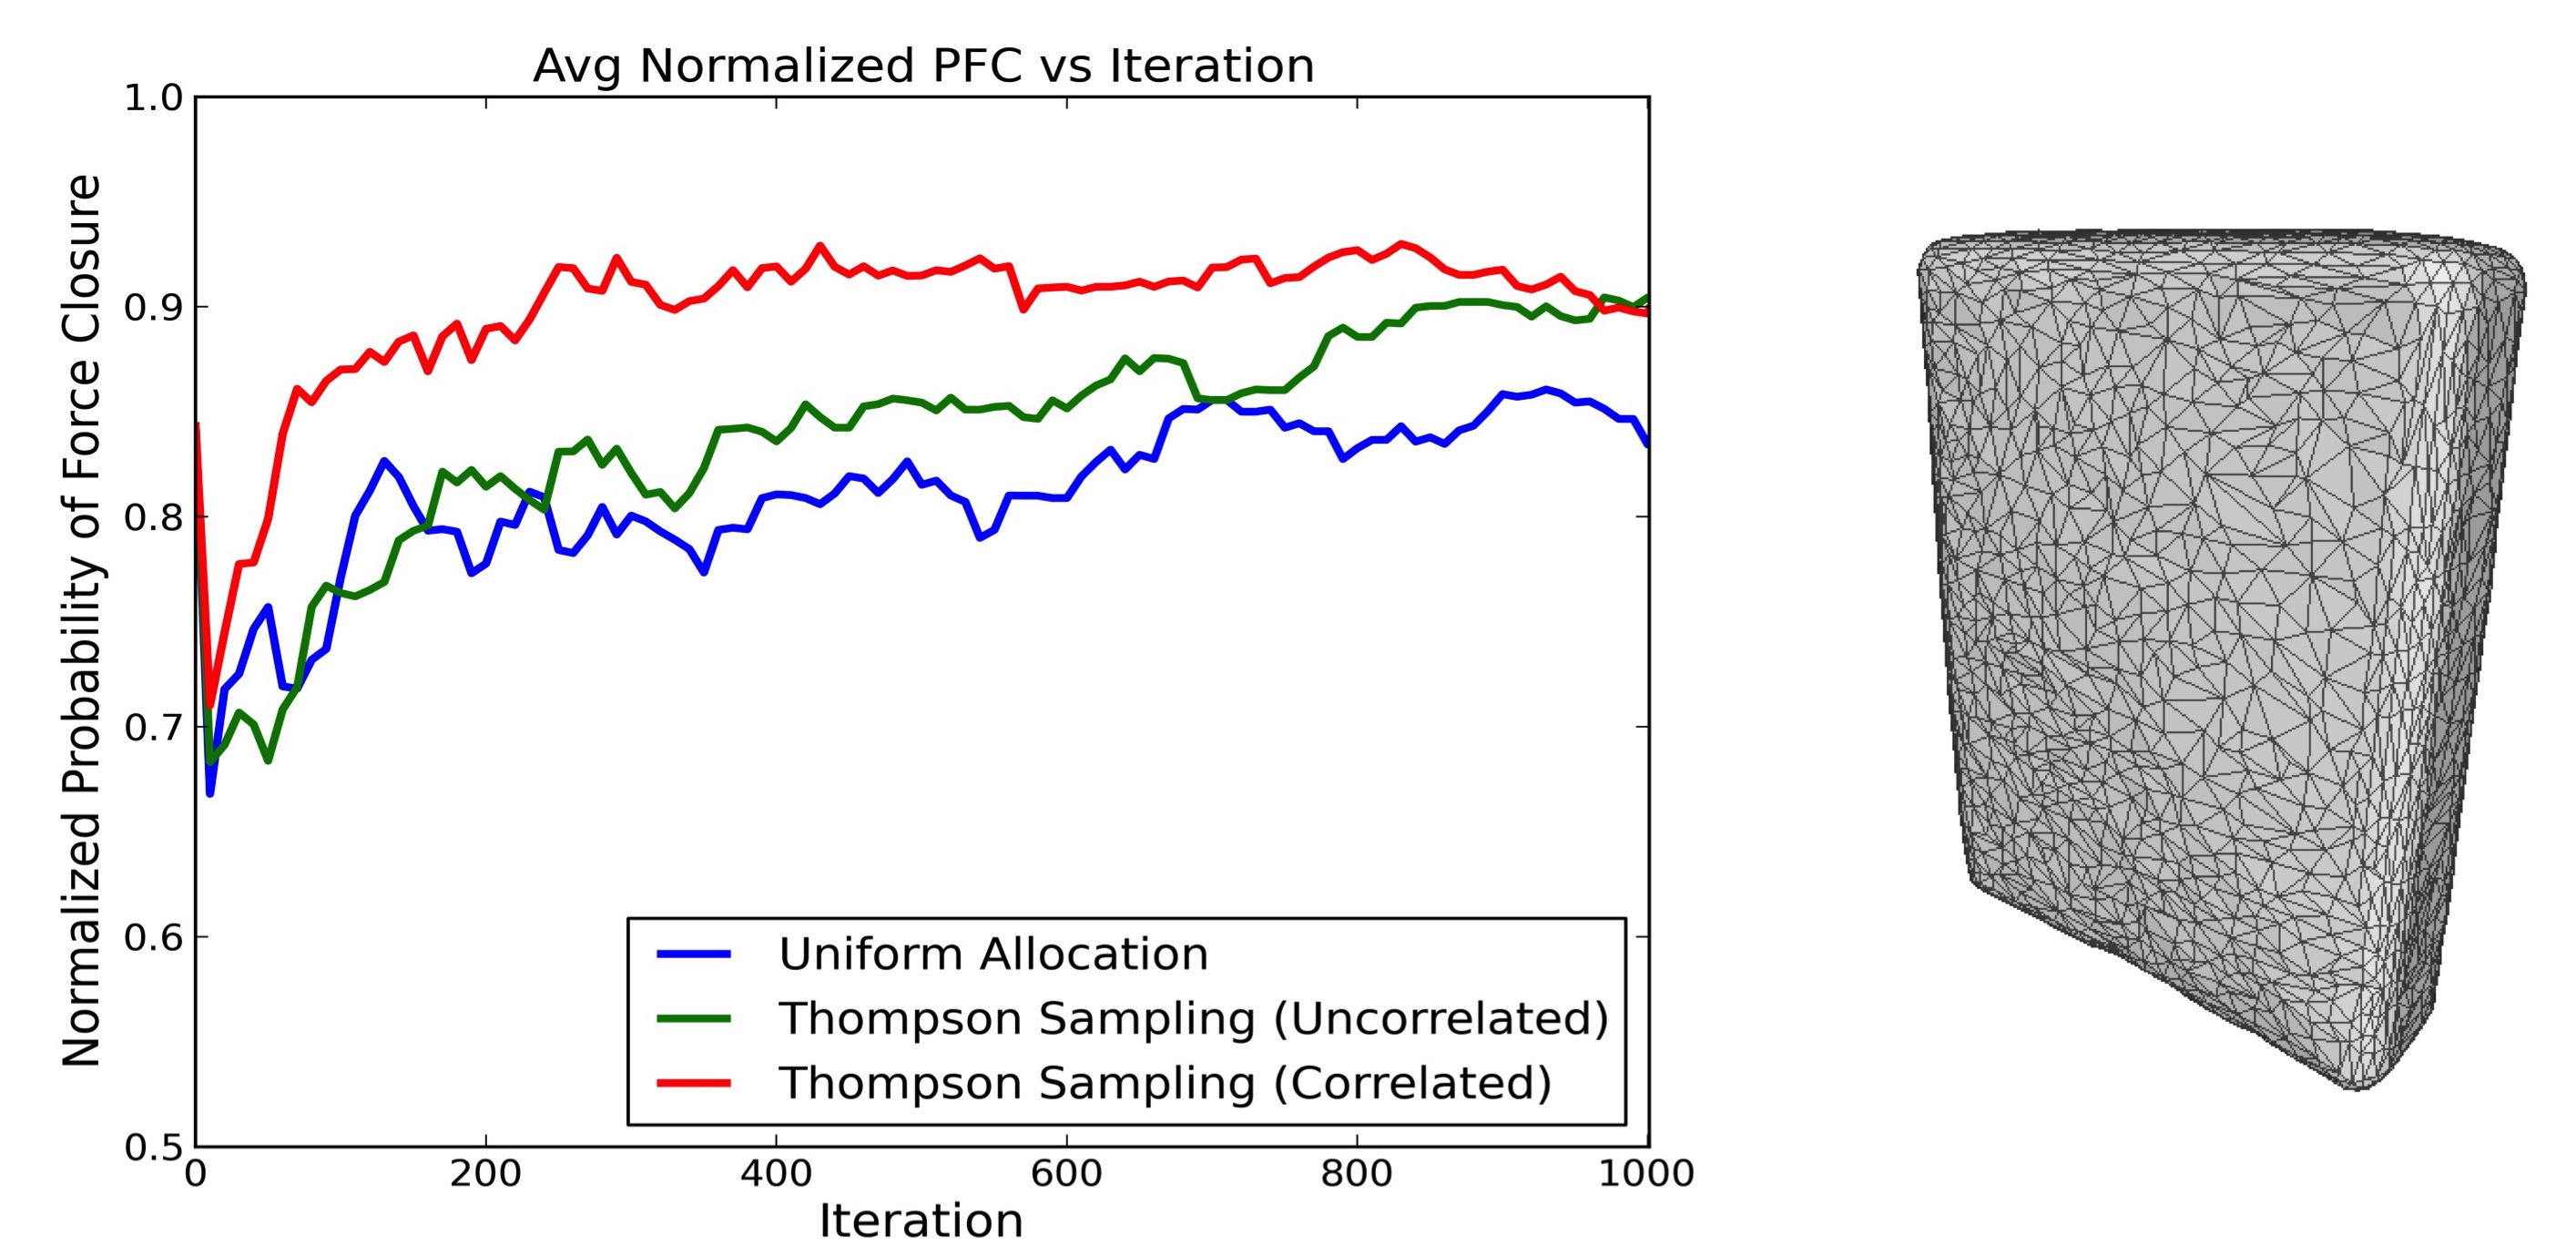
\includegraphics[scale=0.08]{figures/box_avg_reward_w_model.jpg}
        \caption{Normalized $P_F$ on a cereal box with 250 candidate parallel-jaw grasps.}
    \end{subfigure}
    \begin{subfigure}[b]{0.5\textwidth}
        \centering
        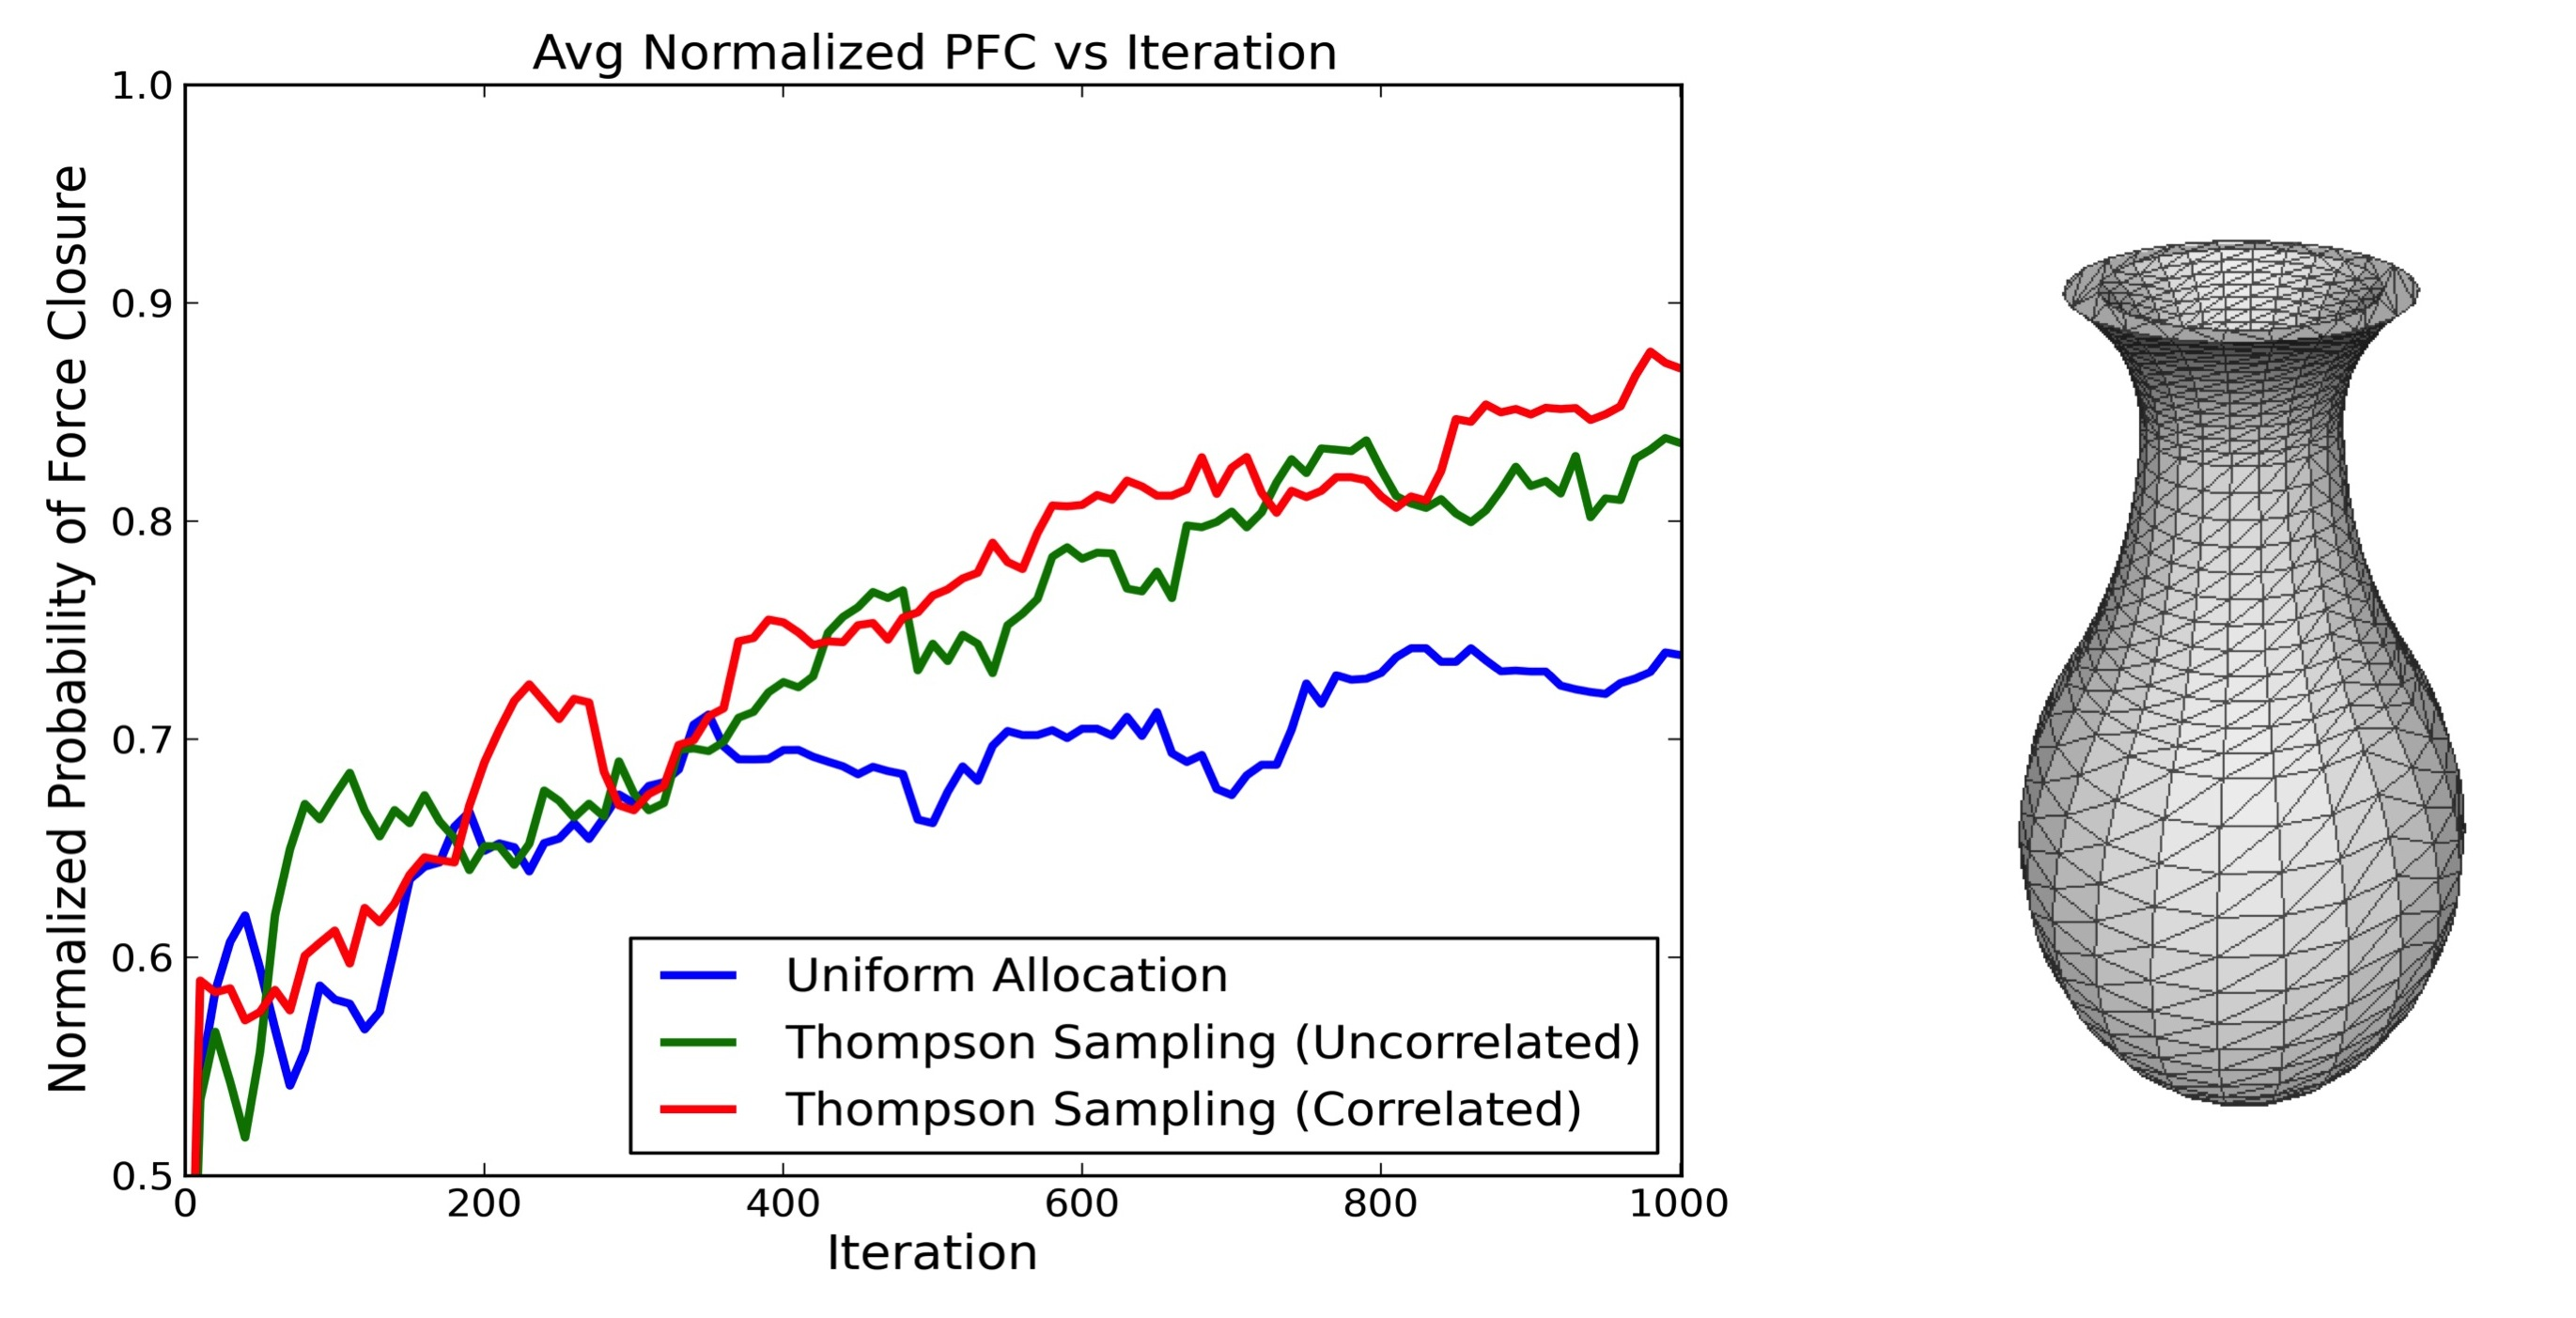
\includegraphics[scale=0.08]{figures/flowerpot_avg_reward_w_model.jpg}
        \caption{Normalized $P_F$ on a flower pot with 250 candidate parallel-jaw  grasps.}
    \end{subfigure}
\caption{Comparison of the normalized $P_F$ of the sampled parallel-jaw grasp versus iteration of the MAB algorithm for correlated Thompson sampling, uncorrelated Thompson sampling, and Uniform Allocation averaged over 20 trials. (a) On the cereal box, correlated Thompson sampling converges to within 90\% of the highest quality grasp approximately 4$\times$ faster than uncorrelated. (b) However, correlated and uncorrelated Thompson sampling perform comparably on the flower pot because there are few grasp similarities in the candidate set. }
\figlabel{local-mab}
\vspace*{-15pt}
\end{figure}

To examine the effects of orders of magnitude of prior data in the MAB algorithms, we ran the algorithms with priors computed from increasingly larger subsets of prior data from Dex-Net: 0, 15, 150, and 1500 objects. 
\figref{global-mab} shows the normalized probability of force closure $P_F$ versus iteration when planning grasps for a bottle and detergent averaged over 50 trials.
For each run of our algorithm, we used prior grasp from the five closest objects in Dex-Net in the multi-view CNN-based shape similiarity vector space.
The objects from Dex-Net were labelled with 250 grasps and $P_F$ evaluated using brute force Monte-Carlo integration.
For the bottle, we see that the convergence of the correlated MAB algorithms to a grasp with high $P_F$ accelerates with increasingly larger subsets of prior data used, and is approximately $10 \times$ faster when using 1500 prior objects.
For the detergent the gains are more modest, with the largest dataset accelerating convergence to within 90\% of the optimal grasp in the set by approximately $1.5 \times$.
As illustrated in \figref{bottle-nn}, the nearest neighbor objects become increasingly similar to the object to label with increasing sizes of datasets from Dex-Net.
This suggests that more prior data may also lead to more similar objects to rarer categories such as the detergent bottle, which may accelerate convergence 
\TODO{Remove}
Future work will examine these effects on a larger subset of objects and will use assitional nearest neighbors from Dex-Net to compute priors.

\begin{figure}[t!]
\centering
\begin{subfigure}[b]{0.5\textwidth}
        \centering
        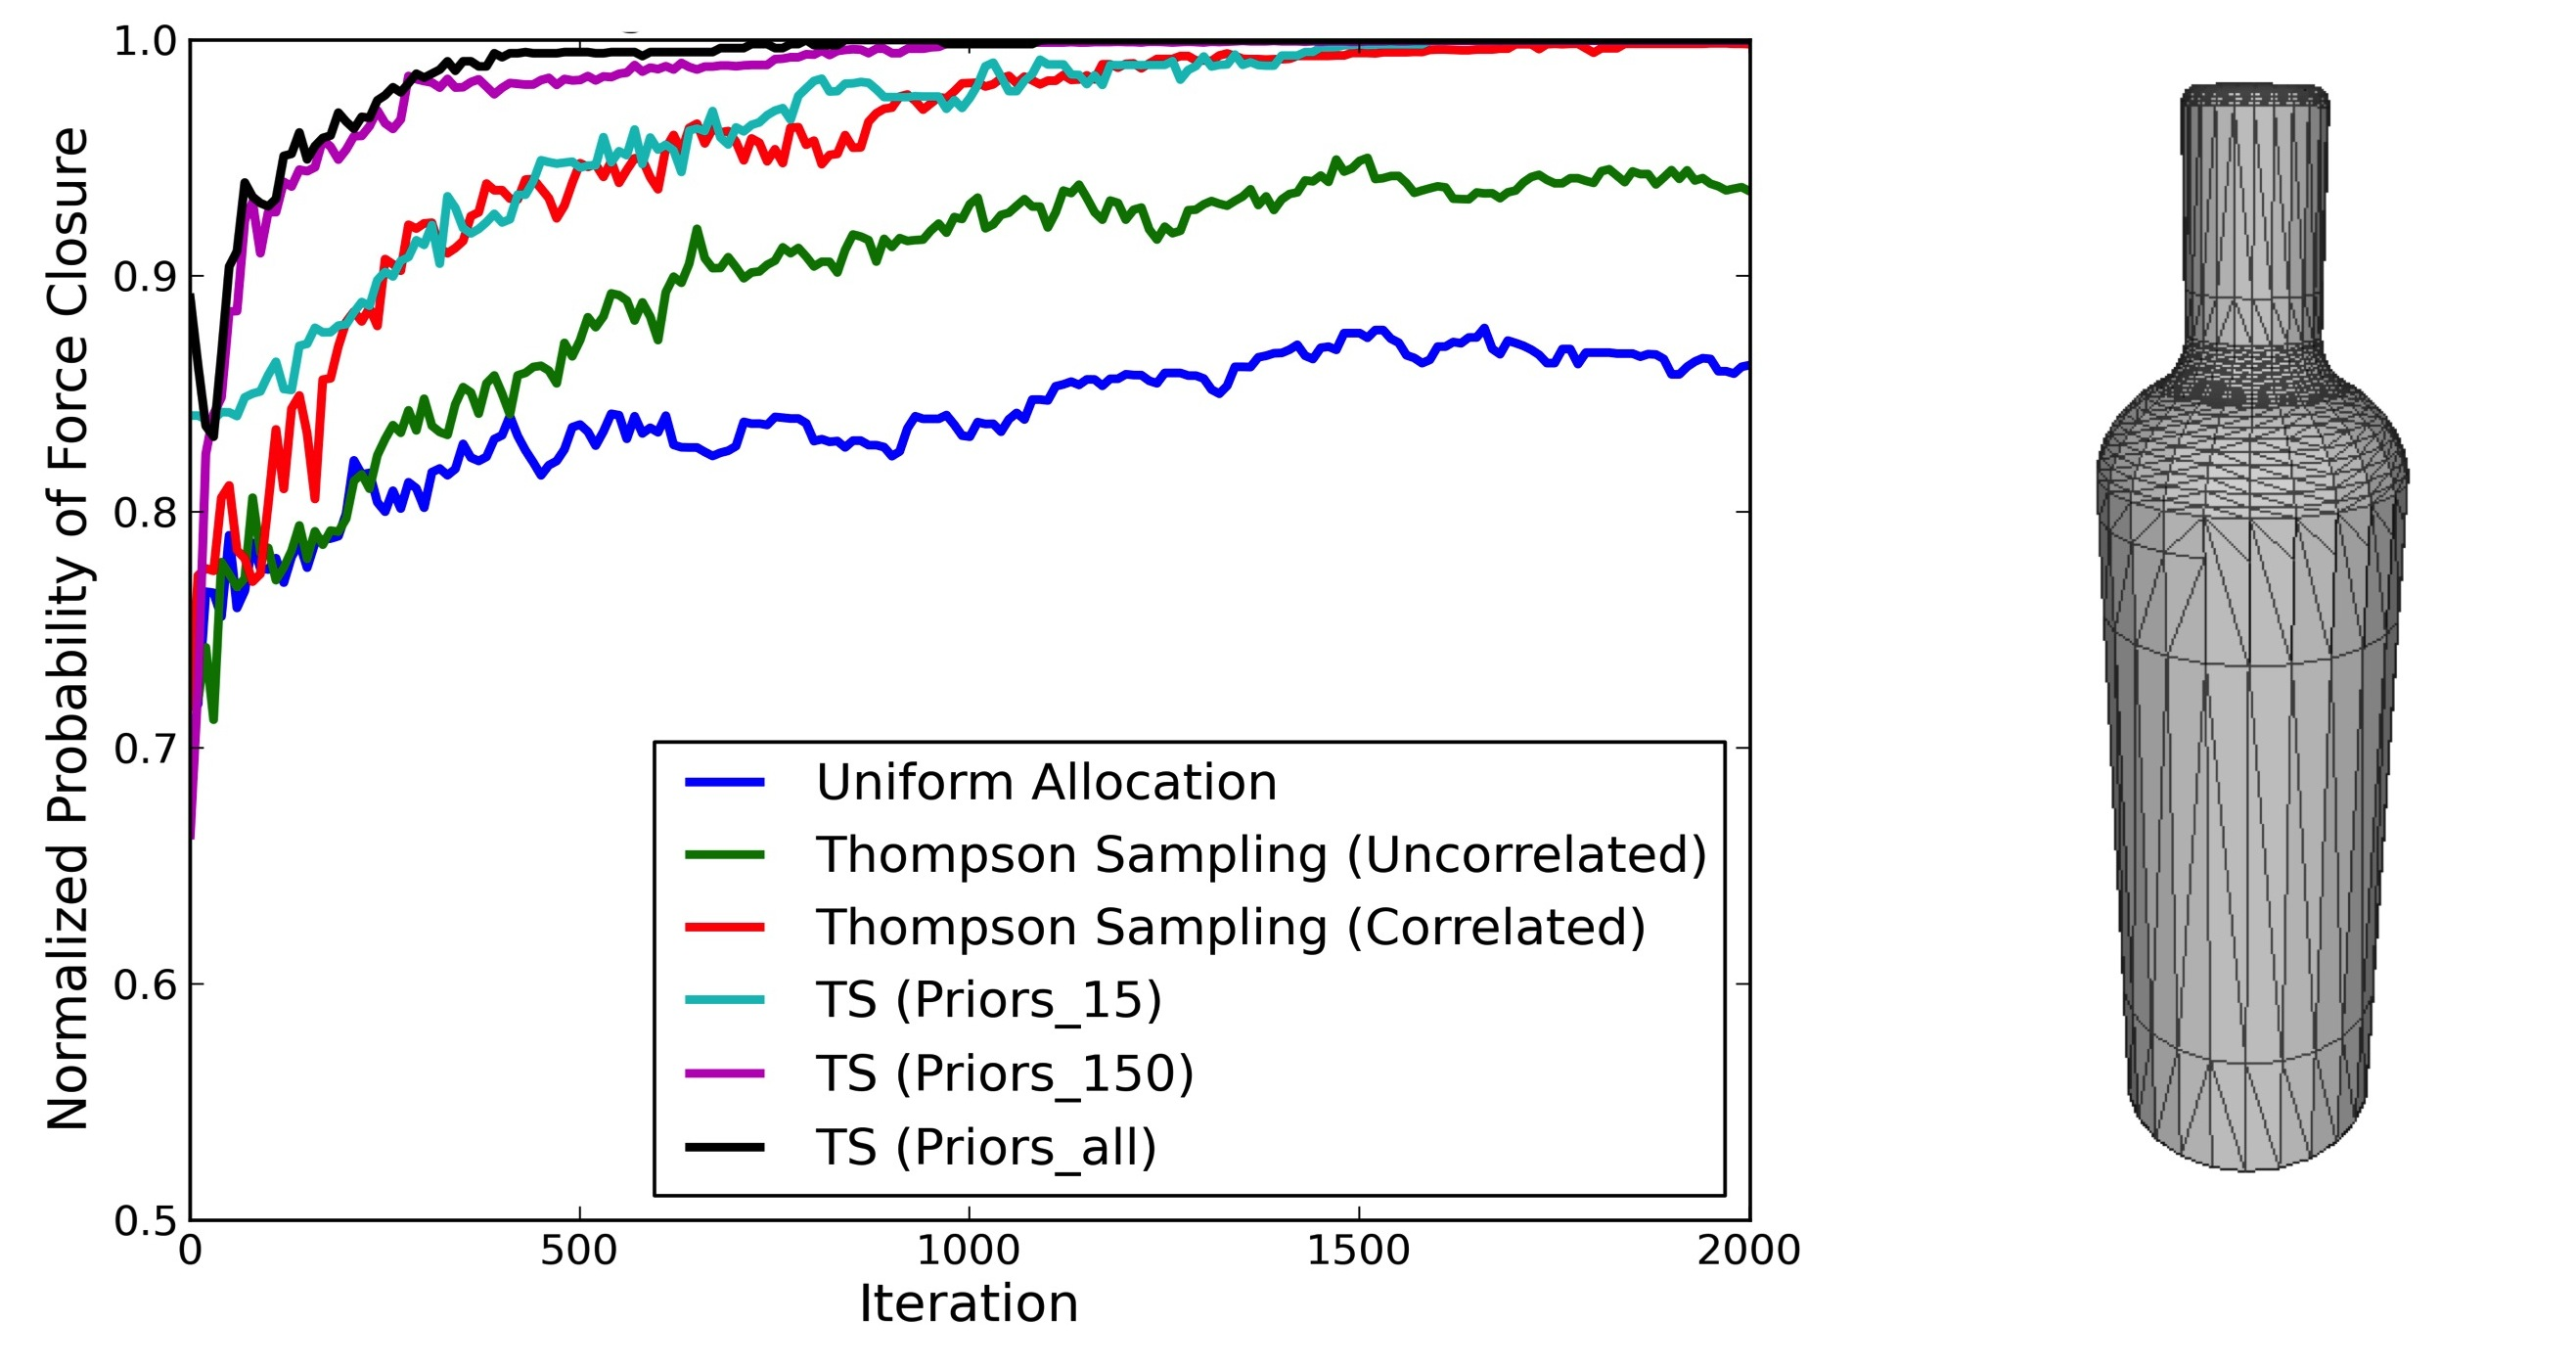
\includegraphics[scale=0.08]{figures/bottle_avg_reward_w_model2.jpg}
        \caption{Normalized $P_F$ on a bottle with 250 candidate parallel-jaw grasps.}
    \end{subfigure}
    \begin{subfigure}[b]{0.5\textwidth}
        \centering
        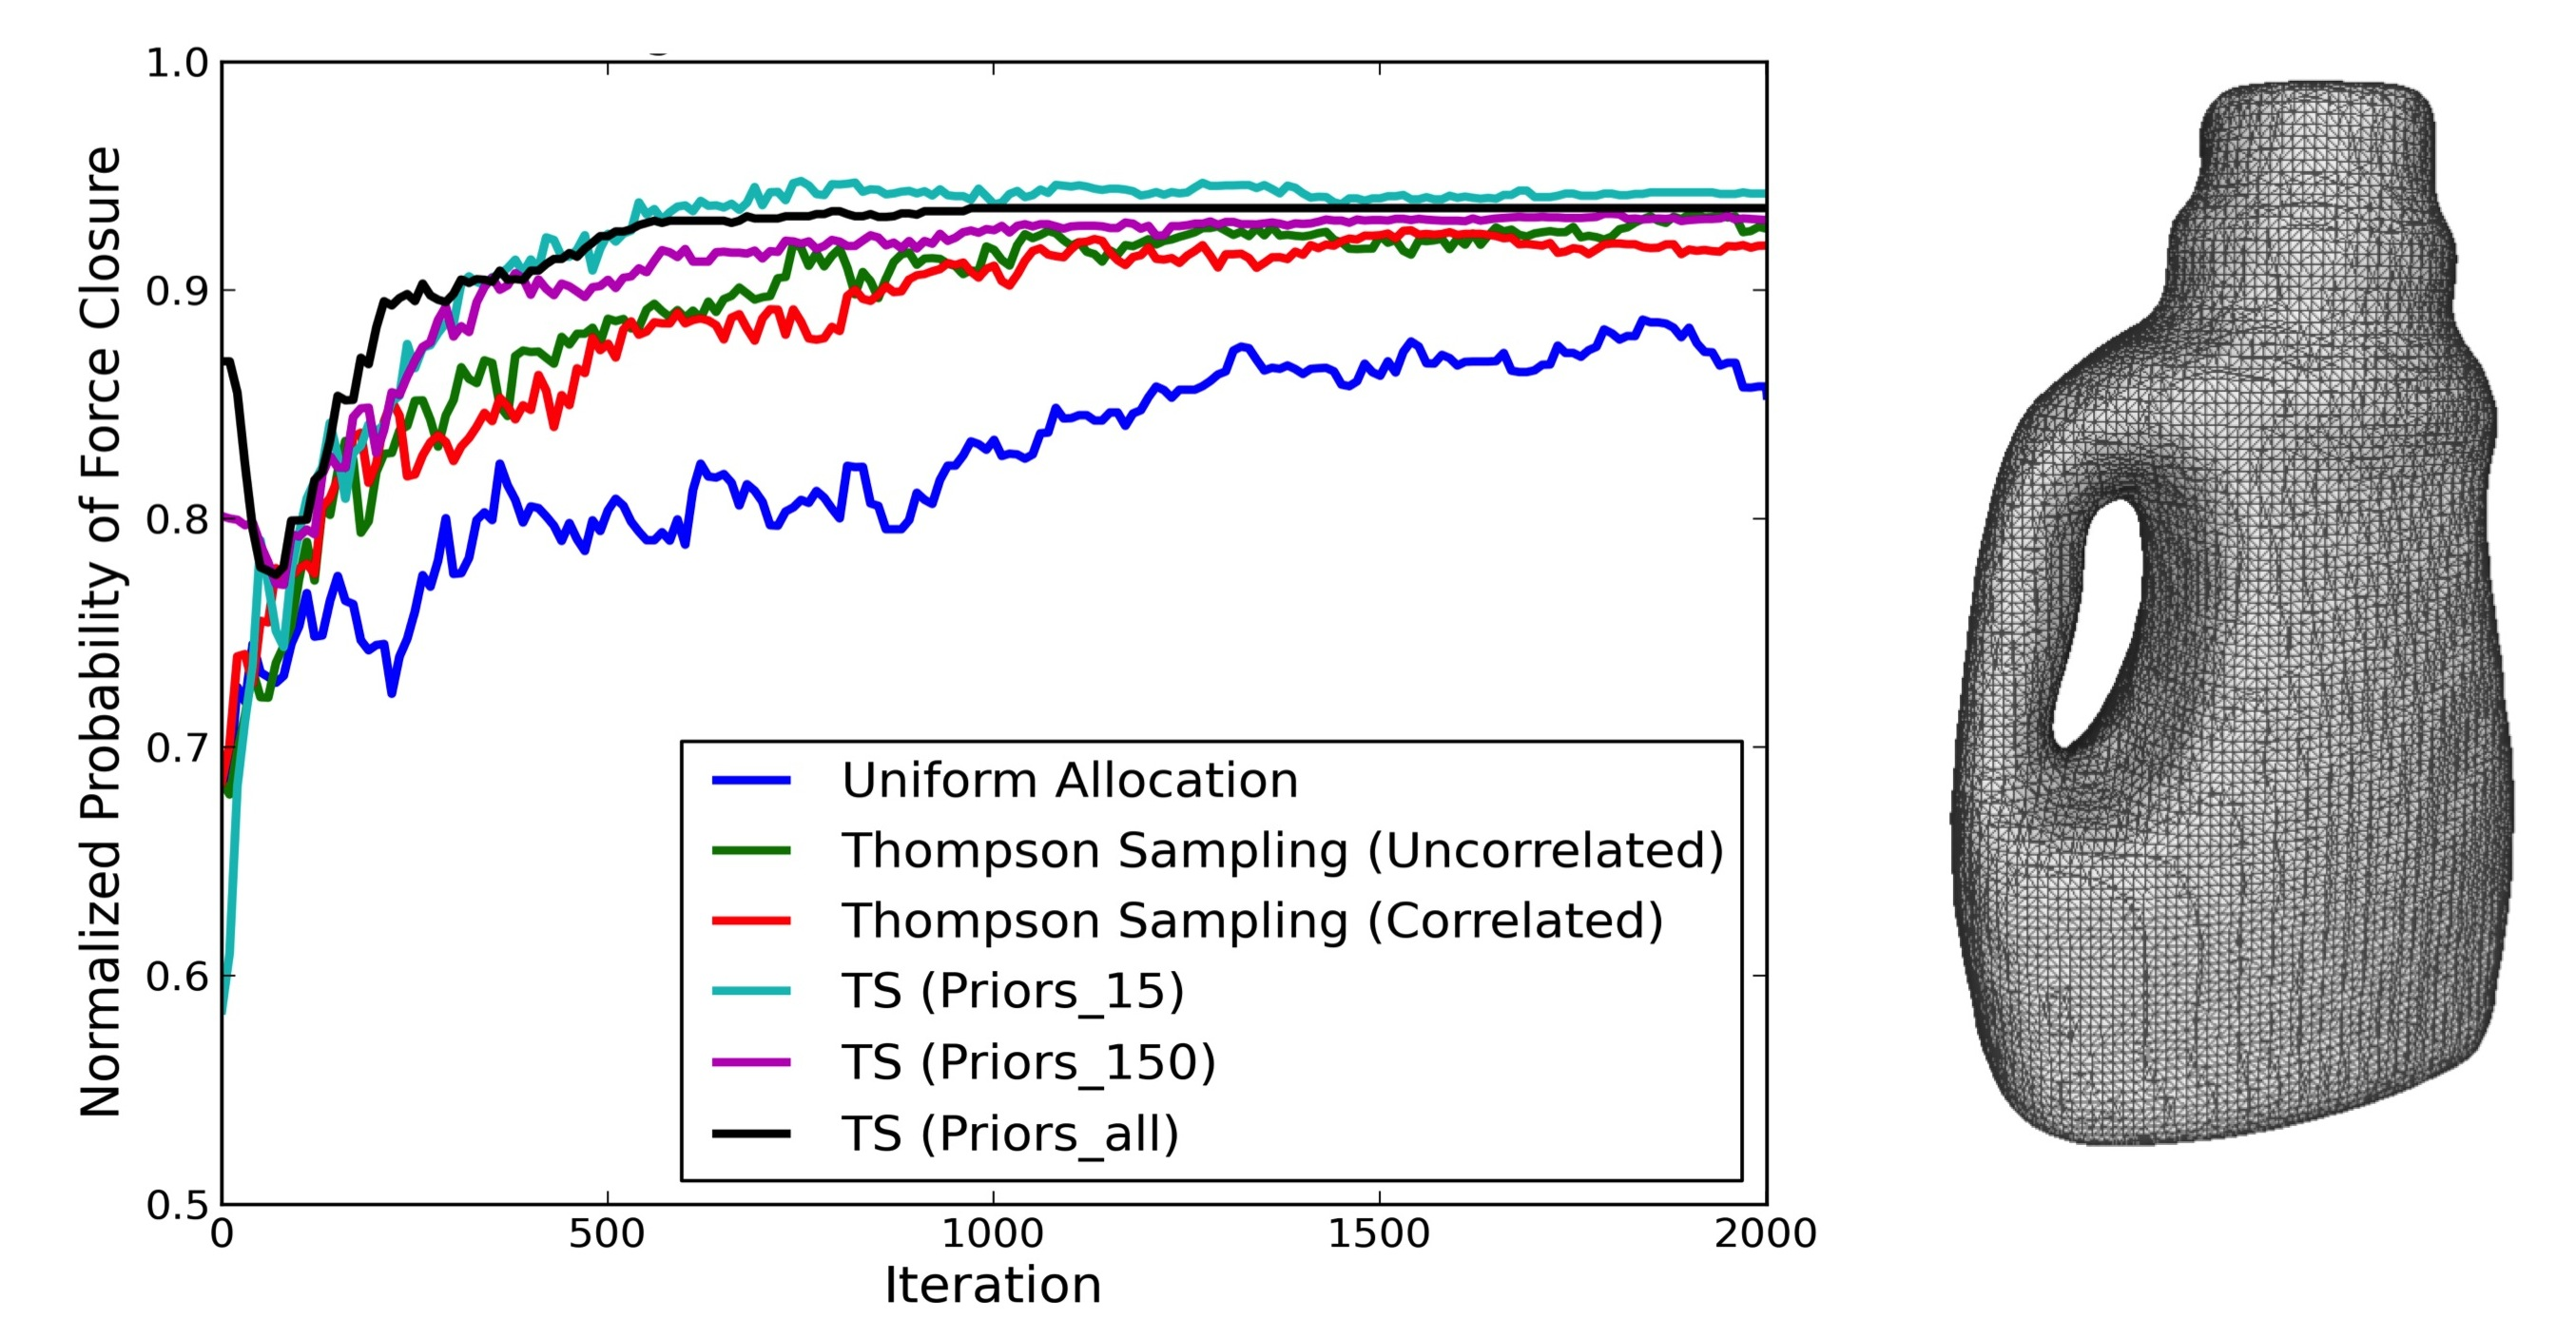
\includegraphics[scale=0.08]{figures/detergent_avg_reward_w_model.jpg}
        \caption{Normalized $P_F$ on a detergent bottle with 250 candidate parallel-jaw grasps.}
    \end{subfigure}
%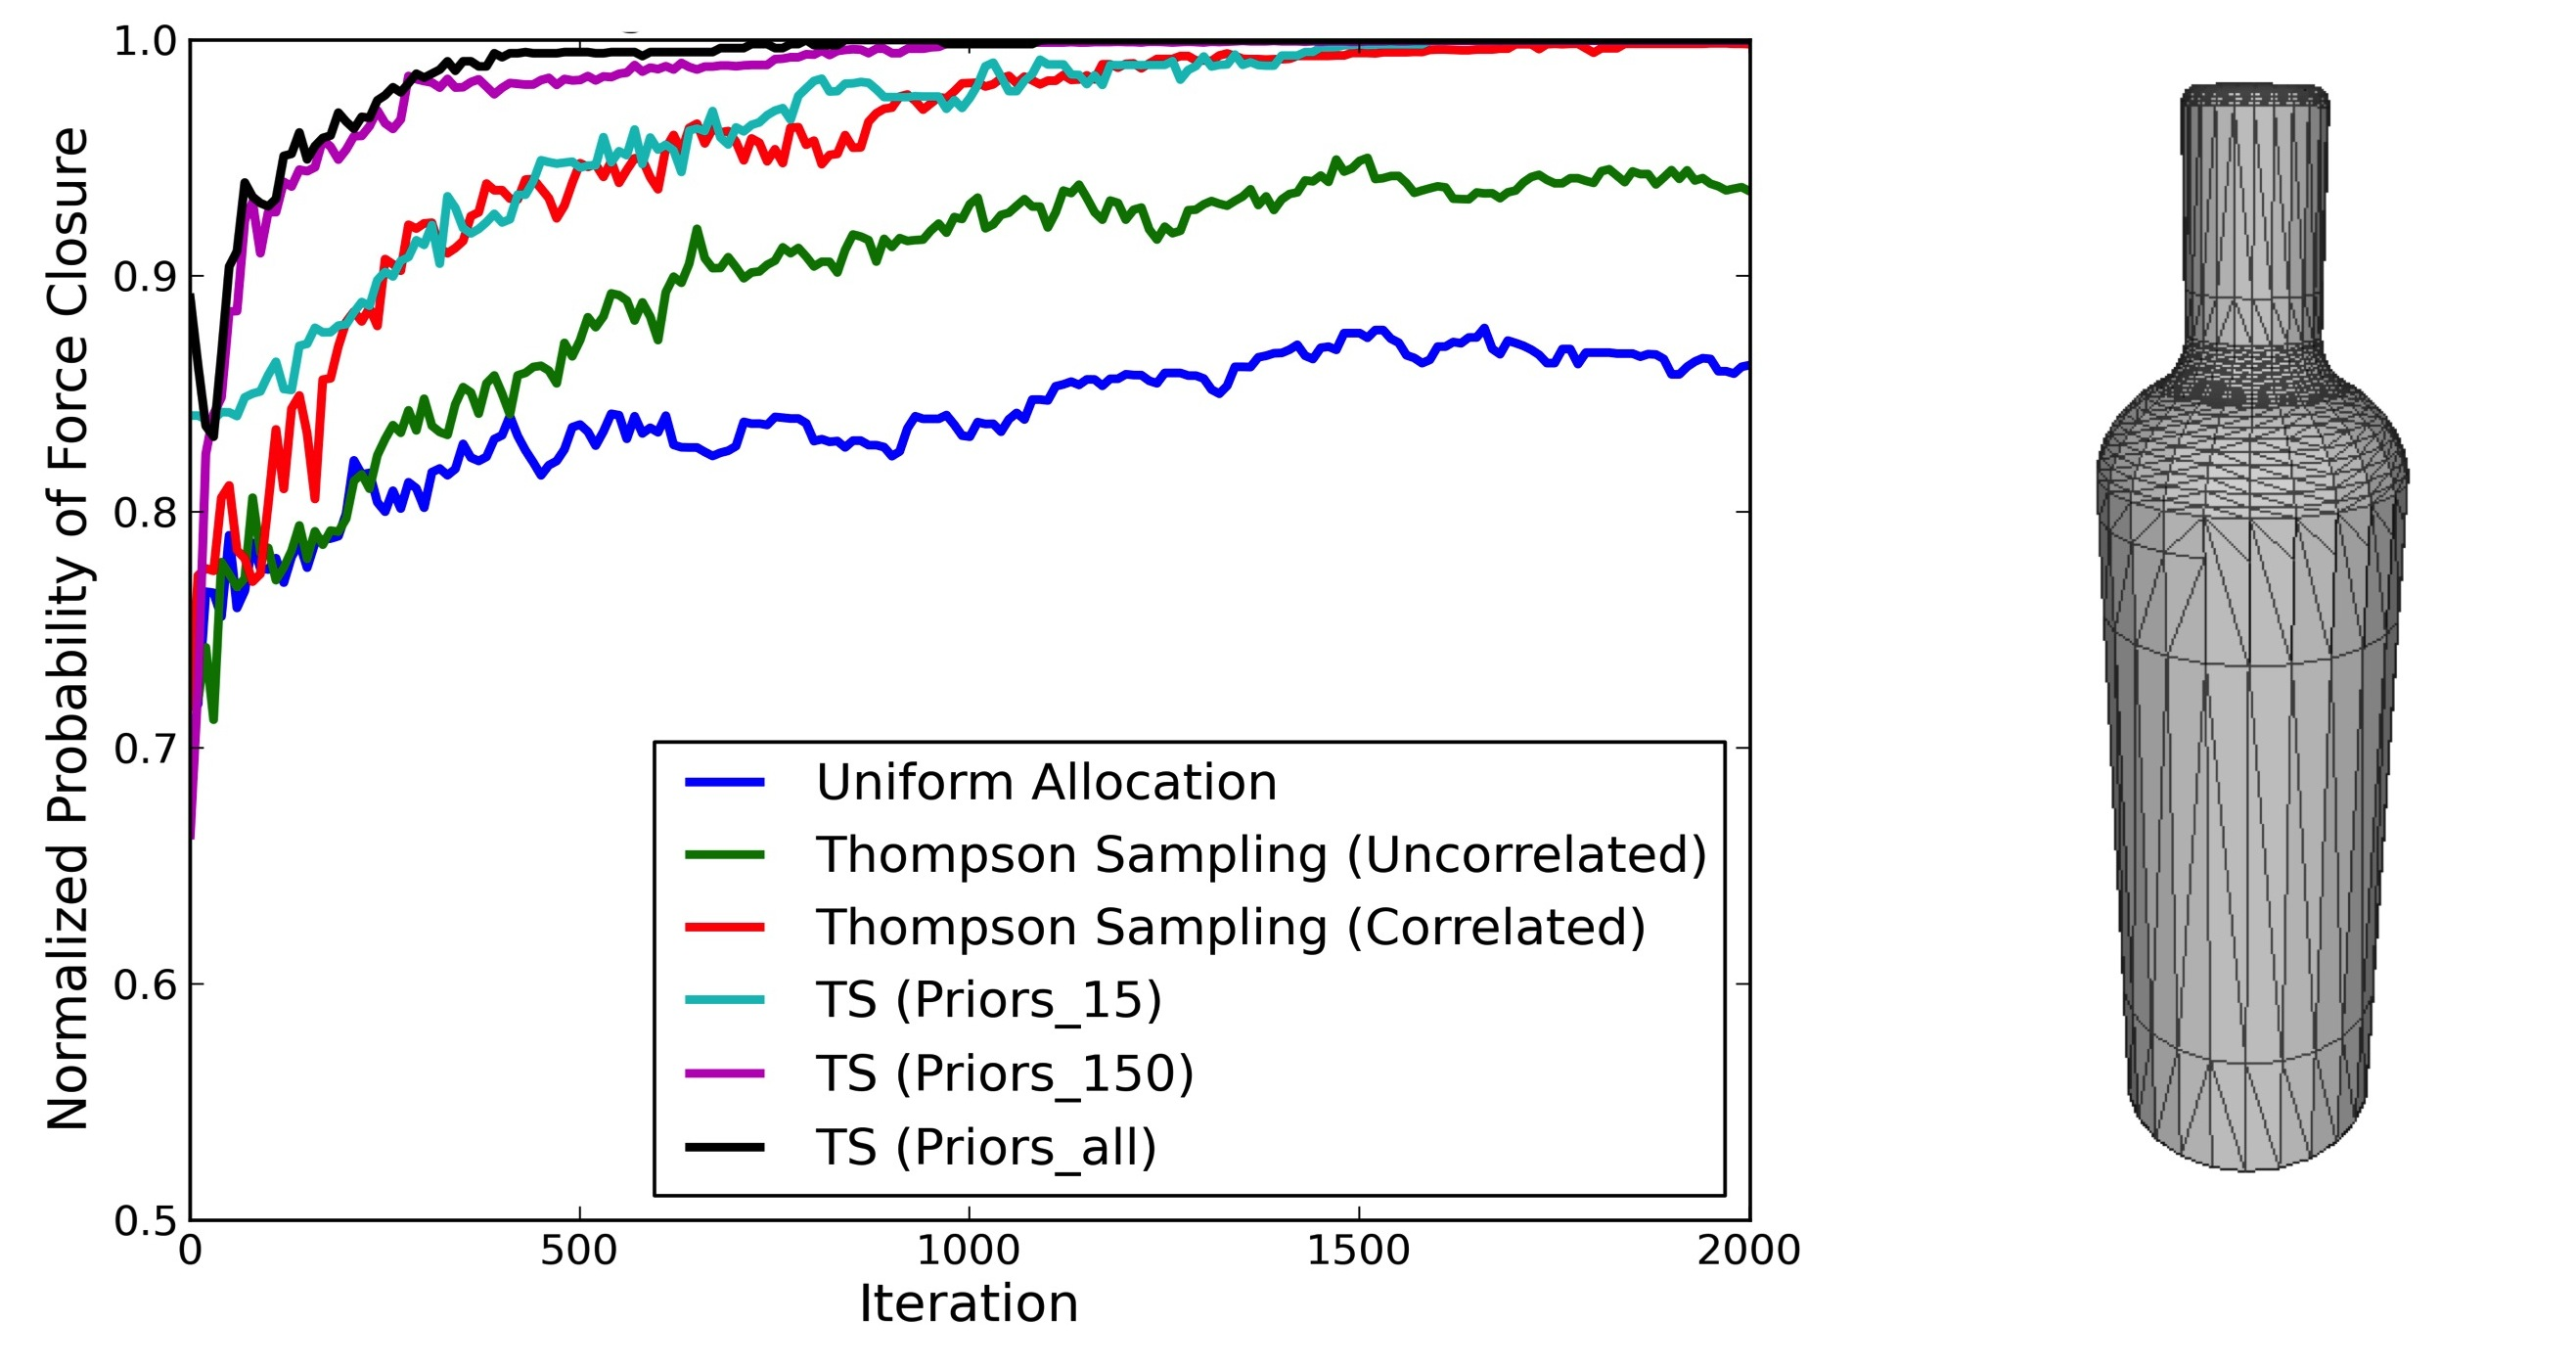
\includegraphics[scale=0.09]{figures/bottle_avg_reward_w_model2.jpg}
\caption{Comparison of the normalized $P_F$ of the sampled parallel-jaw grasp (y-axis) versus iteration of the MAB algorithm (x-axis) for correlated Thompson sampling with and without the use of prior grasps from five nearest neighbors from Dex-Net, uncorrelated Thompson sampling, and Uniform Allocation averaged over 20. Prior grasps were taken from increasingly larger subsets of Dex-Net: 15, 150, and 1500 objects. For the bottle, convergence to within 90\% of the optimal grasp is accelerated by approximately 10$\times$ over uncorrelated Thompson sampling, and performance appears to improve with increasing sizes of the prior dataset used. The detergent converges slightly faster with more prior data, however the speedup is approximately $1.5\times$ and does not appear to improve with additional data from Dex-Net.}
\figlabel{global-mab}
\vspace*{-15pt}
\end{figure}

\begin{figure}[t!]
\centering
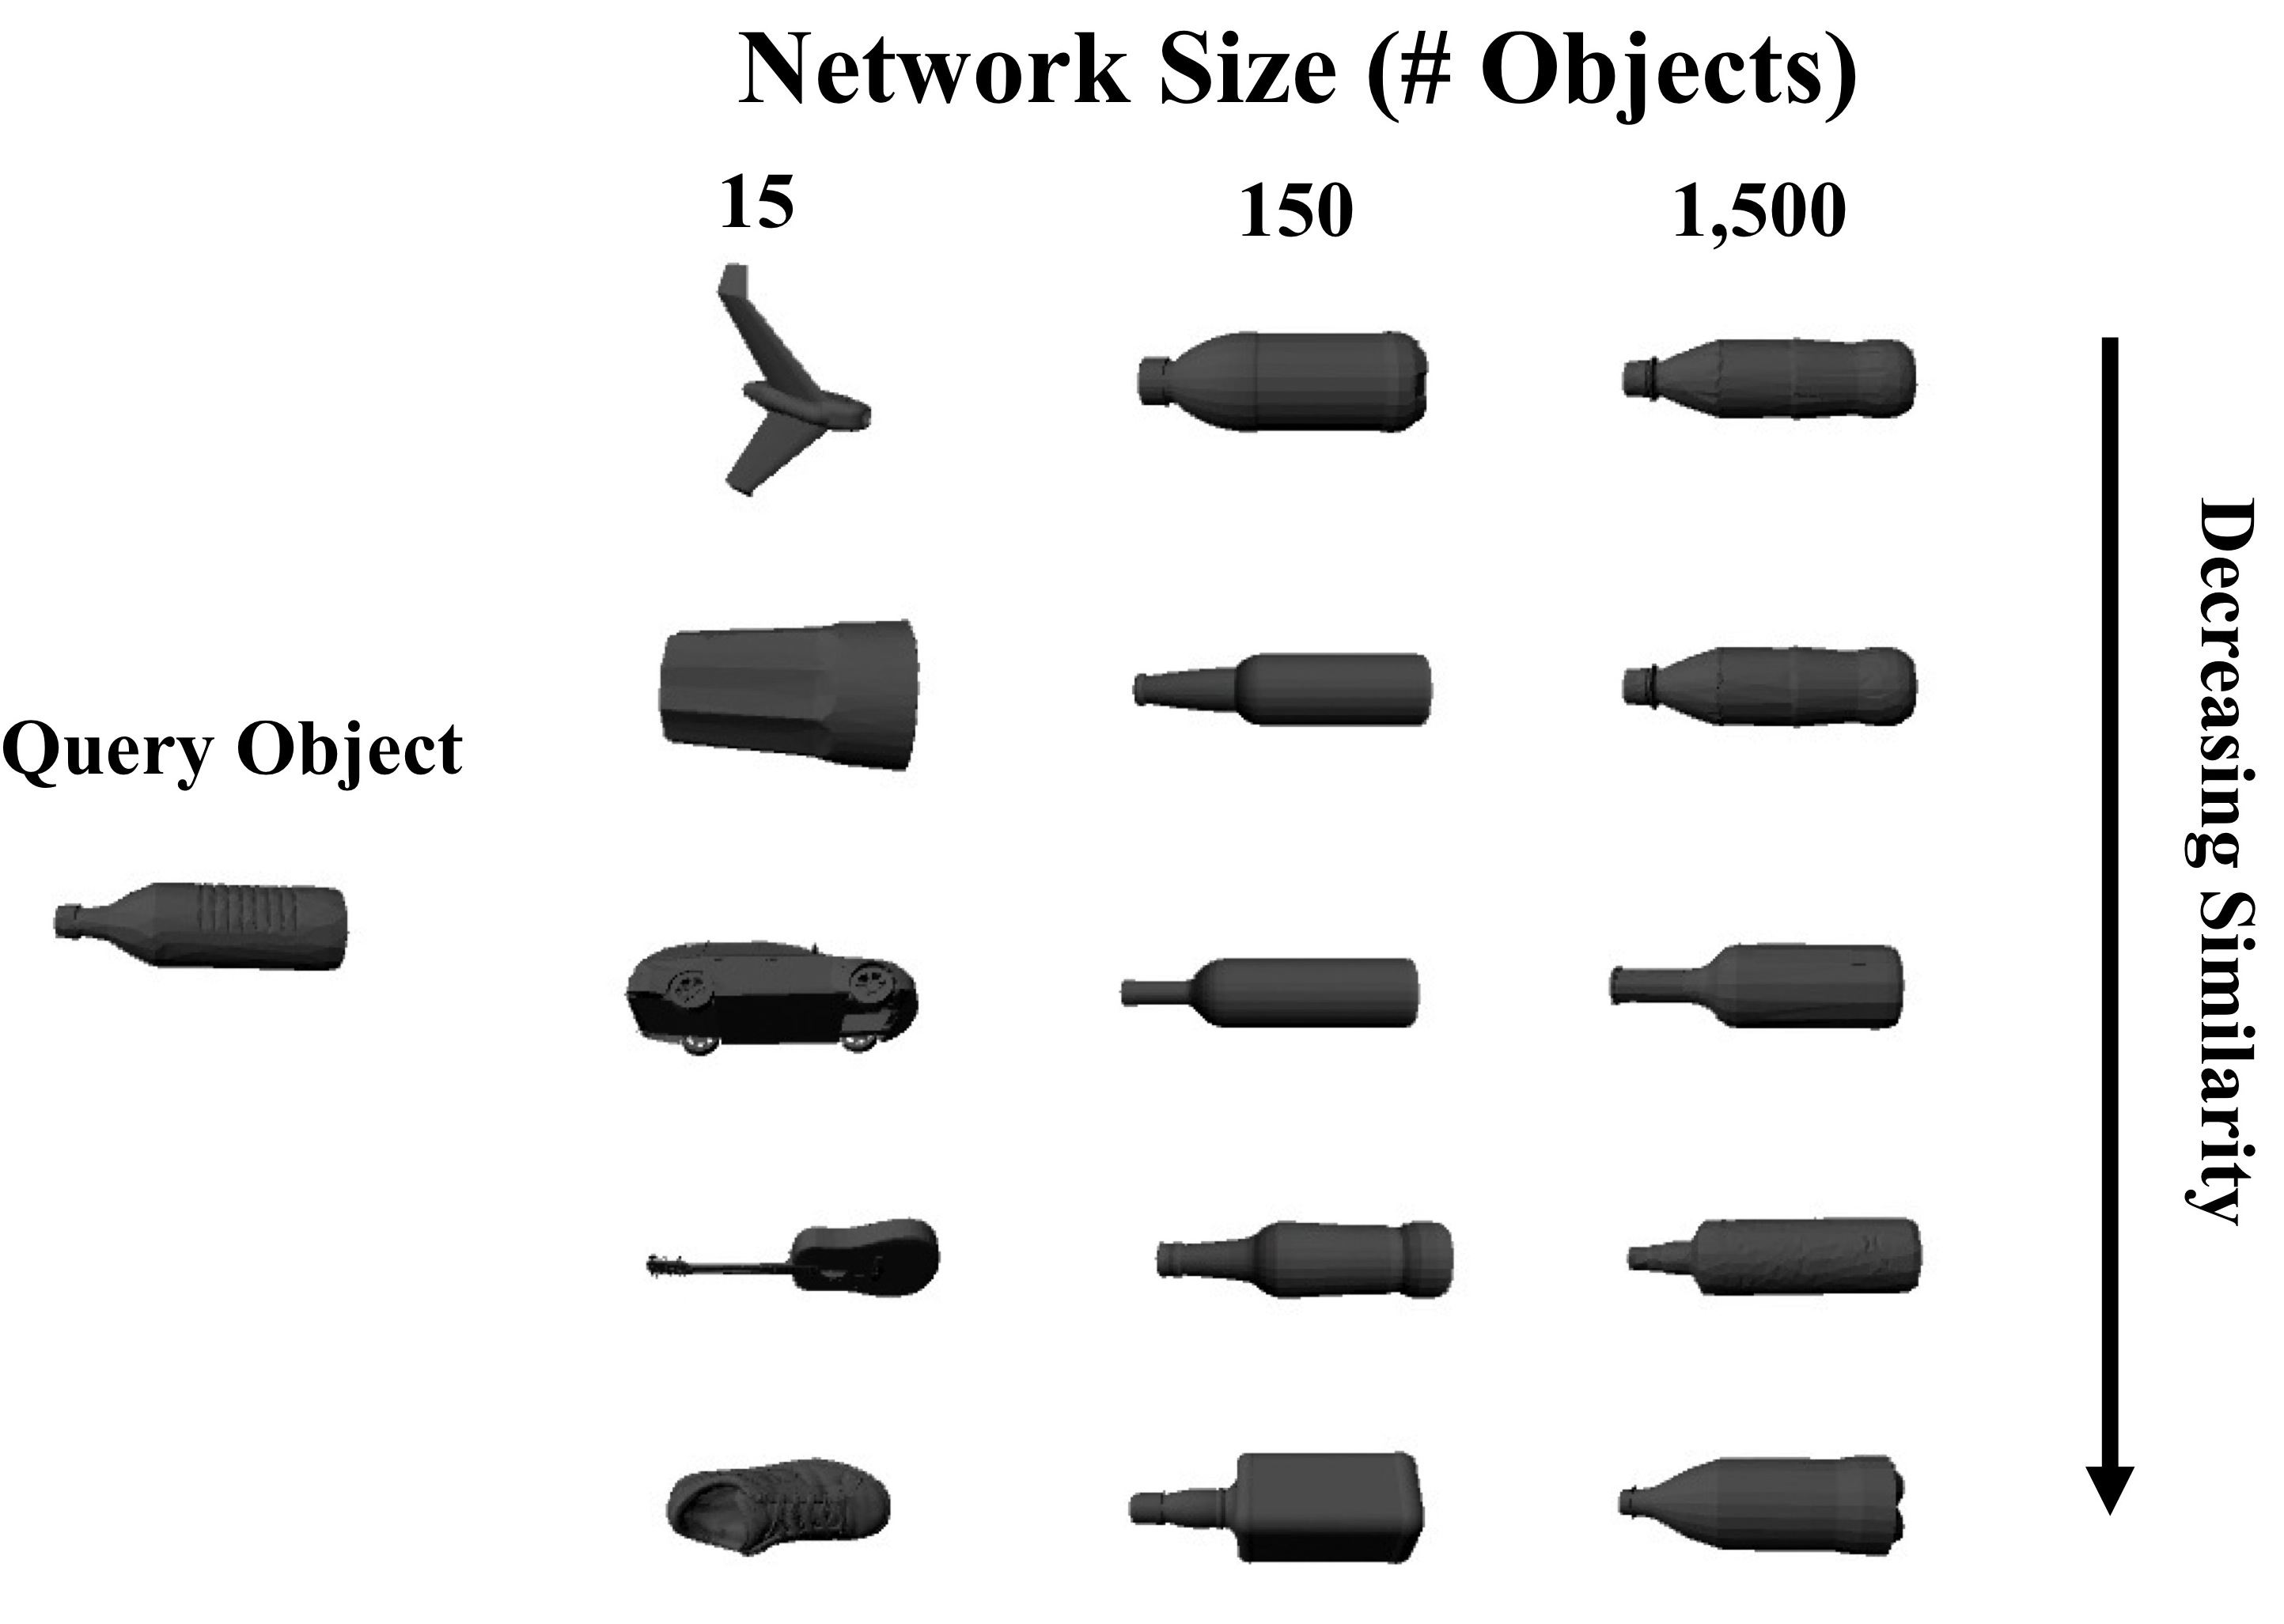
\includegraphics[scale=0.075]{figures/bottle_nearest_neighbors.jpg}
\caption{Illustration of the five nearest neighbor objects from Dex-Net using the multi-view CNN-based shape embedding and Euclidean distance for increasing sizes of randomly selected subsets of data from Dex-Net. We see that while the neighbors for a small dataset are not relevant, the neighbors become increasingly similar to the query bottle as more data is used.}
\figlabel{bottle-nn}
\vspace*{-15pt}
\end{figure}

\section{Sensitivity to Uncertainty}

\TODO{Write section}